\documentclass[a4paper,11pt]{article}

\usepackage[english]{babel}
\usepackage{xcolor}
\usepackage{graphicx}
\usepackage{pdflscape}
\usepackage{outlines}
\usepackage
[
a4paper,
left=2cm,
right=1.5cm,
top=2.5cm,
bottom=2.5cm,
]
{geometry}

% disables automatic identation for all paragraphs, \noindent would be for one specified line
\setlength{\parindent}{0pt}

\usepackage{url}
%\usepackage[showframe]{geometry}

\linespread{1.25}

% using geometry instead
% page layout
%\usepackage{layout}
%\setlength{\voffset}{-1,0cm}
%%\setlength{\hoffset}{-.625in} % 1.875 (10pt standard) - 1.250 (word standard)
%\setlength{\hoffset}{-.450in} 
%\setlength{\headsep}{1cm}
%\setlength{\textwidth}{480pt}
%\setlength{\textheight}{695pt}

%header and footer
\usepackage{fancyhdr}
\usepackage{lastpage}
\pagestyle{fancy}
\fancyhead{}
\lhead{Privilege Escalation on Unix Systems}
\rhead{
\includegraphics[width = 25mm, scale = 0.1]{images/bht-logo}}
\fancyfoot{}
\lfoot{Patrick Rahn - matriculation number: 100927}
\rfoot{Page \thepage\ of \pageref{LastPage}}
\renewcommand{\footrulewidth}{1pt}

% table caption
\usepackage{float}

% enumerate with numbers only
\usepackage{enumitem}

% fancy table
\usepackage{booktabs}

% pictures side by side
\usepackage{subcaption}

% insertin code
\usepackage{listings}

% customize code style
\usepackage{xcolor}

%line break for URLs
\usepackage{xurl}

%pdf inclusion
\usepackage{pdfpages}

\definecolor{codegreen}{rgb}{0,0.6,0}
\definecolor{codegray}{rgb}{0.5,0.5,0.5}
\definecolor{codepurple}{rgb}{0.58,0,0.82}
\definecolor{backcolour}{rgb}{0.95,0.95,0.92}

%Python code style
\lstdefinestyle{mystyle}{
    backgroundcolor=\color{backcolour},   
    commentstyle=\color{codegreen},
    keywordstyle=\color{codepurple},
    numberstyle=\tiny\color{codegray},
    stringstyle=\color{codegreen},
    basicstyle=\ttfamily\footnotesize,
    breakatwhitespace=false,         
    breaklines=true,                 
    captionpos=b,                    
    keepspaces=true,                 
    numbers=left,                    
    numbersep=5pt,                  
    showspaces=false,                
    showstringspaces=false,
    showtabs=false,                  
    tabsize=2
}

\lstset{style=mystyle}

% HTML code style
\lstdefinestyle{MyHTML}{
    backgroundcolor=\color{backcolour},   
    commentstyle=\color{codegray},
    keywordstyle=\color{orange},
    numberstyle=\tiny\color{codegray},
    stringstyle=\color{codegreen},
    basicstyle=\ttfamily\footnotesize,
    breakatwhitespace=false,         
    breaklines=true,                 
    captionpos=b,                    
    keepspaces=true,                 
    numbers=left,                    
    numbersep=5pt,                  
    showspaces=false,                
    showstringspaces=false,
    showtabs=false,                  
    tabsize=2
}

%JavaScript language
\lstdefinelanguage{JavaScript}{
  keywords={typeof, new, true, false, catch, function, return, null, catch, switch, var, if, in, while, do, else, case, break},
  keywordstyle=\color{blue}\bfseries,
  ndkeywords={class, export, boolean, throw, implements, import, this},
  ndkeywordstyle=\color{darkgray}\bfseries,
  identifierstyle=\color{black},
  sensitive=false,
  comment=[l]{//},
  morecomment=[s]{/*}{*/},
  commentstyle=\color{purple}\ttfamily,
  stringstyle=\color{red}\ttfamily,
  morestring=[b]',
  morestring=[b]"	
}

%JavaScript Style
\lstdefinestyle{MyJS}{
    backgroundcolor=\color{backcolour},   
    commentstyle=\color{codegray},
    keywordstyle=\color{orange},
    numberstyle=\tiny\color{codegray},
    stringstyle=\color{codegreen},
    basicstyle=\ttfamily\footnotesize,
    breakatwhitespace=false,         
    breaklines=true,                 
    captionpos=b,                    
    keepspaces=true,                 
    numbers=left,                    
    numbersep=5pt,                  
    showspaces=false,                
    showstringspaces=false,
    showtabs=false,                  
    tabsize=2
}

% urls
\usepackage{hyperref}

\begin{document}
\includepdf[pages =1]{cover/ewp_project_cover.pdf}
% page numbering
\pagenumbering{arabic}
\tableofcontents
\setcounter{secnumdepth}{4}
\setcounter{tocdepth}{4}
\newpage
%enumerate with numbers only
\renewcommand{\labelenumii}{\arabic{enumi}.\arabic{enumii}}
\renewcommand{\labelenumiii}{\arabic{enumi}.\arabic{enumii}.\arabic{enumiii}}
\renewcommand{\labelenumiv}{\arabic{enumi}.\arabic{enumii}.\arabic{enumiii}.\arabic{enumiv}}

%-----Start of the Document-----

\section{Introduction}

\subsection{Context}

Privilege escalation is common tactic in the context of cyber attacks. It is a collection of various techniques which all aim to achieve gaining higher-level permissions on a system or network. Initially adversaries find a way to enter and explore a network even irrespective of the fact they only have unprivileged access. In most cases this not sufficient for the overarching goals and elevated permissions are required to follow through on the actual objectives. \newline\newline Common ways to achieve this is through exploiting system weaknesses and misconfigurations. The desired end result is to have elevated access in from of root level, local administrator or an account with admin-like access.\footnote{The Mitre Cooperation. Privilege Escalation [online] homepage: attack.mitre.org URL: https://attack.mitre.org/tactics/TA0004/ [Accessed 26.11.2025]}

\subsection{Problem statement}

The Berliner Hochschule für Technik (BHT) is one the largest state universities of applied sciences in Germany.  It was founded in 1971 and it offers a wide range of bachelor and master courses. It runs its own data center which encompasses  many different technologies spanning different hardware vendors, operating systems and software applications. The university has several machines which run Unix operating systems of various distributions. The machines vary in setup and configuration. This heterogeneous technical landscape can accumulate a plethora of misconfigurations over time. Some of them may lead to serious vulnerabilities including insecure permissions, shell escapes and kernel exploits. \newline At the moment there is no comprehensive tool or script in place which can detect misconfigurations and provide the necessary information to mitigate vulnerabilities.  \newline\newline This can lead to severe consequences concerning the safety of the network infrastructure of the university. It leaves the door open for various damaging scenarios including complete loss of data or extortion through a ransomware attack. 

\subsection{Research Objectives}

The aim is to identify the misconfigurations and other aspects on Linux machines which could cause vulnerabilities. \newline\newline First it has to be established which systems are actually part of the university network and are using a Linux distribution as the operating system. Next the relevant systems are scanned for misconfigurations. Furthermore once the vulnerabilities have been detected and verified solutions will be suggested in order to mitigate them. 

\subsection{Research Questions}

The thesis aims to answer the following questions:

\begin{itemize}
	\item Which misconfigurations are prevalent on Linux machines?
	\item Which vulnerabilities can result from the misconfigurations that have been found?
	\item What are the solutions to mitigate the vulnerabilities?
\end{itemize}

\subsection{Significance and Benefits}

There are a plethora of tools which scan systems for monitoring reasons or detecting vulnerabilities. These are often big applications with a graphical user interface and a steep learning curve. They need to cover a lot of different options and systems. I propose a lean but effective CLI (command line interface) tool which narrows down on finding misconfiguration on Linux systems. The approach is to get satisfying results through a simple CLI which takes very minimal effort to understand and use. Most importantly I further propose using eBPF (extended Berkeley Packet Filter) to detect misconfigurations behaviorally not just statically. \newline\newline To address the aforementioned questions I have developed CLI tool which detects misconfigurations statically and behaviorally, uses these to identify potential vulnerabilities and gathers further information through connecting to APIs to improve the security of the affected systems. \newline To this end, I make the following contributions:

\begin{enumerate}
	\item comprehensive but user-friendly CLI
	\item thoroughly analyzing how the system is configured (static approach)
	\item use eBPF to observe runtime behavior
	\item kernel surface checks via eBPF probes
	\item collecting useful information through retrieving information from CVE APIs
\end{enumerate}

\subsection{Scope and Limitations}

The tool is designed to scan for misconfigurations only on systems which run a Linux distribution for the operating system. There will be no graphical user interface. It is solely a CLI tool. \newline It finds misconfigurations, lays out potential vulnerabilities and suggests techniques to mitigate those. It is not designed to change any wrong configurations. Furthermore it has no capability to automate changing configurations on the machines. \newline\newline There is no notification system in place which notifies the user over email or phone. The script will run and the results will displayed on screen and optionally written into a PDF file. 

\subsection{Structure of the Thesis}

The second chapter 'Technical Base' will go through all the relevant technologies and tools which are used together to make up this project. \newline\newline The third chapter 'Analysis' defines the requirements for the tool. It covers functional, technical and security related aspects. \newline\newline The fourth chapter 'Design' depicts how the tool fulfills the requirements laid out in the 'Analysis' chapter. Some topics are system architecture, component design and UML diagrams. \newline\newline The fifth chapter 'Implementation' show how the design has been translated into working code. It explains what was built and how and what challenges arose in the process. \newline\newline The sixth chapter 'Utilization' demonstrates how the tool is actually used. It shows the real-world usage, effectiveness of the tool and most importantly how it solves the problems identified beforehand. \newline\newline The seventh chapter 'Evaluation' provides proof that the tool works and assesses its quality. Moreover it reflects on how well it meets the defined goals. 

\subsection{AI Usage}

AI was used for these specific tasks:

\begin{itemize}
	\item finding appropriate literature
	\item finding appropriate research papers
	\item guiding and helping to refine the structure of the thesis when necessary
	\item assisting in understanding complex topics
\end{itemize}







\section{Technical Base}

\subsection{Unix-based Operating Systems}

The Unix-based operating systems are a family of operating systems. They all have one thing in common which is that they share the design principle of the original Unix System. Unix was developed in Bell Labs and its predecessor was the Multics system \cite{farrow1991}.  The core characteristics of the Unix system are that it is a general-purpose, interactive and multi-user operating system \footnote{Dennis M. Ritchie and Ken Thompson. The UNIX Time-Sharing System [online] homepage: dsf.berkeley.edu URL: https://dsf.berkeley.edu/cs262/unix.pdf [Accessed 28.11.2025]}.

\subsection{Linux}

\subsubsection{General Aspects}

Linux is an open-source operating system based on Unix. The Linux kernel was created by Linus Torvalds and was first released back in 1991. Linus Torvalds had a kernel but no additional programs like a shell and compilers which together comprise a working system. Richard Stallman and GNU provided the needed programs and together the first version of the Linux operating system was created \footnote{What is Linux. [online] homepage: linux.org URL: https://linux.org/threads/what-is-linux.4106/ [Accessed 28.11.2025]}. Linux is comprised of several different components including the bootloader, kernel, Init system. daemons, graphical server, desktop environment and applications. \footnote{The Linux Foundation. What is Linux? [online] homepage: linux.com URL: https://www.linux.com/what-is-linux/ [Accessed 28.11.2025]}

\subsubsection{Kernel}

The kernel is the core of the operating system. It is the central software which has various critical responsibilities. It first and foremost manages and allocates computer resources like CPU, RAM and devices. It is the connecting tissue between hardware and software and consequently allows users to manage system components like networks, file systems and drivers among other things. \newline\newline The most important tasks performed by the kernel are listed below:

\begin{itemize}
	\item Process scheduling
	\item Memory management
	\item Provision of a file system
	\item Creation and termination of processes
	\item Access to devices
	\item Networking
	\item Provision of a system call application programming interface (API)
\end{itemize}

A very significant concept in this context is the distinction between user mode and kernel mode. Different processes have different rights. A user process should never access kernel addresses. Modern systems including Linux use a split virtual address space. Virtual memory is marked as either being part of user space or kernel space. As a result while CPU is running in user mode it can only access memory which is marked as being in the user space. \newline\newline  Kernel mode is the highest privilege level. There are operations which can only be performed while the CPU is in kernel mode as the operation needs access to memory which is in the kernel space. These operations need access and right to resources a user mode operation should never have. Typical examples of such operations include system call processing and accessing memory-management hardware \cite{kerrisk2010}.

\subsubsection{Daemons}

Daemons are special processes. They are background processes to be more specific, which means they run continuously without direct user interaction as they have no controlling terminal. Many of them are started when the system boots and continues running until the system is shut down\cite{kerrisk2010}.

\subsubsection{Shell}

The shell is also referred to as command interpreter because it captures its functionality. It is a program which acts as an interface between the user and operating system. The user can type in commands which will be executed programs in response to the user's commands. \newline\newline Bash (Bourne again shell) is the commonly used shell on Linux systems. Shells are not just designed for interactive use. Another important feature are shell scripts, which are text files containing shell commands\cite{kerrisk2010}.

\subsubsection{Filesystem}

A filesystem is comprised of serveral components which all put together give it the functionality it needs to do its job\footnote{David Both. An introduction to Linux's EXT4 filesystem. [online] homepage: opensource.com URL: https://opensource.com/article/17/5/introduction-ext4-filesystem [Accessed 29.11.2025]}.

\begin{enumerate}
	\item Data storage: organized collection of files and directories to store and retrieve data
	\item Namespace: methodology which provides rules for naming and organizing data in a hierarchy
	\item Security model: a scheme for defining access rights
	\item API: a set of system calls for navigating and manipulating objects like directories and files
	\item Implementation: software to tie the filesystem components together.
\end{enumerate}

The kernel supports many diverse implementations of filesystems \cite{nemeth2011}. All these filesystems differ in certain aspects of their implementation for example concerning how blocks are allocated or the organization of directories. However programs can not be written in a way to account for all the implementations of filesystems. The virtual file system (VFS) is a kernel feature which provides a solution for this conundrum by creating an abstraction layer for filesystem operations. The concept is a two-way as the VFS defines a generic interface for filesystem operations and in turn each filesystem an implementation of the interface\cite{kerrisk2010}.\newline\newline The default and thereby most common used filesystem on many Linux distributions is ext4 \footnote{Bosko Marijan. Linux File System: Types, Features, Limitations. [online] homepage: phoenixapp.com URL: https://phoenixnap.com/kb/linux-file-system [Accessed 29.11.2025]}.



\setcounter{secnumdepth}{4}
\paragraph{Everything is a file}

 "In Linux everything is a file." is a common phrase. It actually refers to the fact that all system resources like processes, hardware and network connections are represented as files and can be accessed using standard file operations. A file system is commonly divided into data blocks for storing file content and inodes for storing metadata and pointers to the data blocks. Inodes hold the information for any Linux file with the exception of the file's name and data \footnote{Linux basic concepts [online] homepage: microsoft.github.io URL: https://microsoft.github.io/WhatTheHack/020-LinuxFundamentals/Student/resources/concepts.html [Accessed 28.11.2025]}.

\setcounter{secnumdepth}{4}
\paragraph{Single Directory Hierarchy}

It is the responsibility of the kernel to organize all files in the system. In Linux the kernel achieves this by maintaining a single hierarchical directory structure where at its base resides the root directory which is named '/' (slash) \cite{kerrisk2010}. The following picture shows a subset of this single directory hierarchy.

\smallskip
\begin{figure}[h]
\centering
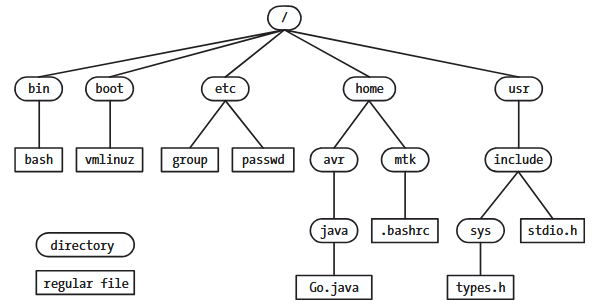
\includegraphics[scale=1, keepaspectratio]{images/single-directory-hierarchy}
\caption{Single Directory Hierarchy \cite{kerrisk2010}}
\end{figure}

\setcounter{secnumdepth}{4}
\paragraph{File Types}

The Linux filesystem has seven file types which are listed below\cite{nemeth2011}:

\begin{itemize}
	\item Regular files
	\item Directories
	\item Character device files
	\item Block device files
	\item Local domain sockets
	\item Named Pipes (FIFOs)
	\item Symbolic links
\end{itemize}

\subsubsection{Distributions}

Linux distributions are also referred as distros and are complete operating systems built on the Linux kernel. A distro includes the kernel, system tools, packet manager bundled with all the other necessary components to be ready for use out of the box. There are hundreds of distros available today, each come with a pre-installed set of programs and each customized to target a different user audience\footnote{Gavin Wright. What is Linux distros (Linux distribution)? [online] homepage: techtarget.com URL: https://www.techtarget.com/searchdatacenter/definition/Linux-distros-Linux-distribution [Accessed 29.11.2025]}.

\subsection{Python}

\subsubsection{General Aspects}

Python is a high-level and interpreted programming language and was created by Guido van Rossum. An interpreter is a program which reads and executes line by line or statement by statement. This contrary to a compiler which translates the entire source code into object code before being executed \cite{downey2012}.  \newline\newline It is a strongly, dynamically typed language. This means that it has a strict type system but variables are in essence simply pointers objects. Objects have a permanent type however variables can point to arbitrary objects.  It is a very versatile language and therefore used in wide array of different fields including web development, automation, data science and artificial intelligence among many others. 

\subsubsection{Scripting Language}

Python is an advanced scripting language which posses high-level data structures. In application scripting the functionality of another program is expanded and is often used in context of automation. Furthermore it is used to interact with the operating system or language binding wrappers in which the code libraries are used to bridge two different languages thereby allowing a library written in one language to be used from another.

\subsubsection{Python and Unix/Linux}

The script to scan Linux machines is written in Python. Below a table of Python libraries used to interact with the Linux operation system in order to find out all the necessary information about the machine to evaluate its status regarding the risks for privilege escalation. \newline

\begin{tabular}{@{} *5l @{}}    \toprule
\emph{Purpose} & \emph{Library}   \\\midrule
Executing Commands & subprocess \\
Filesystem inspection & os, pathlib, shutil \\
Regex parsing & re \\
Process interrogation & os, /proc parsing \\
Serialization & json, pickle, csv\\\bottomrule
 \hline
\end{tabular}

\subsubsection{Command Line Interface}

The goal is to create a more advanced command line interface to facilitate all the required options and ensure a great user experience. The choice for the appropriate library fell on \textit{click}. It offers advanced features such as decorator-based approach to defining commands, automatic argument validation and reusable commands\footnote{Usool. Mastering Command-Line Interfaces (CLI) in Python: A Comprehensive Guide. [online] homepage: dev.to URL: https://dev.to/usooldatascience/mastering-command-line-interfaces-cli-in-python-a-comprehensive-guide-10bc [Accessed 29.11.2025]}. Moreover it capable of handling file handling out of the box and supports implementation of Unix/POSIX command line conventions\footnote{Why Click? [online] homepage: click.palletsproject.com URL: https://click.palletsprojects.com/en/stable/why/ [Accessed 29.11.2025]}.

\subsubsection{BCC - BPF Compiler Collection}

It is a framework for creating eBPF programs which are embedded inside a python a program. The eBPF programs are written in C and BCC features bindings for Python \footnote{BPF Compiler Collection (BCC). [online] homepage: github.com URL: https://github.com/iovisor/bcc [Accessed 30.11.2025]}.


\subsection{Understanding Vulnerabilities}

This section will exam vulnerabilities in context of privilege escalation. We examine the vulnerability and lay out which operating system components are involved, how they are work and why the misconfigurations can lead to the vulnerabilities in the first place. 

\subsection{CVEs API}

The National Institute of Standards and Technology (NIST) provides an API which can be used to retrieve information about CVEs (Common Vulnerabilities and Exposures) from the NVD (National Vulnerability Database)\footnote{NIST. National Vulnerability Database. [online] homepage: nvd.nist.gov URL: https://nvd.nist.gov/developers/vulnerabilities [Accessed 30.11.2025]}. Once a vulnerability is found this service can provide additional information and guidance on how to handle the findings and identifying possible solutions to mitigate the risks. 

\subsection{eBPF}

eBPF stands for extended Berkeley Packet Filter. It is a technology which allows users to run sandboxed programs with privileged access within the Linux kernel without modifying the kernel's source code. Users can write eBPF programs to extend the capabilities of the operating system at run time.  It enables a wide range of applications, including advanced networking, security, and observability \footnote{eBPF Documentation - What is eBPF. [online] homepage ebpf.io URL: https://ebpf.io/what-is-ebpf/ [Accessed 30.11.2025]}. 

\section{Analysis}

\subsection{Introduction}

!

\subsection{Current Situation}

!

\subsection{Objectives}

!

\subsection{Functional Requirements}

!

\subsection{Non-functional Requirements}

!

\subsection{Security Requirements}

!

\subsection{Technical Requirements}

!

\subsection{Stakeholder Analysis}

!

\subsection{Constraints and Limitations}

!

\section{Design}

\subsection{Introduction}

The design chapter goes through the various design choices. It explains the architecture and components among other aspects. At the end of the chapter has justifications for the most important parts of the design and its limitiations.\newline\newline The goal is to implement the requirements which were determined in the analysis phase.

\subsection{User Stories}

\begin{enumerate}
	\item As a system admin I want to scan the system for misconfigurations in order to reduce the vulnerability of the system.
	\item As a system admin I want to diagnose the behavior of my system during runtime using eBPF.
	\item As a system admin I want to choose which mode (static, behavior, both) I want to use for a particular scan.
	\item As a system admin I want to decide the type of output of the scan.
\end{enumerate}

\subsection{System Architecture}

\subsubsection{Separation of Concerns}

The most important aspect which is the base for any software architecture is Separation of Concerns (SoC) \footnote{Ralf Westphal. IODA Architecture. [online] homepage: ralfwestphal.substack.com URL: https://ralfwestphal.substack.com/p/ioda-architecture [Accessed 08.01.2026]}. It is a fundamental design principle in software engineering, involving the division of a system into distinct sections, where each section handles a specific, separate "concern" or responsibility. The aim is to produce more maintainable, understandable, and flexible code by minimizing overlap and interdependence between all the parts \footnote{Okay Tonka. What Is Separation Of Concerns? [online] homepage: medium.com URL: https://medium.com/@okay.tonka/what-is-separation-of-concern-b6715b2e0f75 [Accessed 08.01.2026]}.

\subsubsection{High-Level - Conceptual View}

There are four layers needed from a high-level view point.

\smallskip
\begin{figure}[h]
\centering
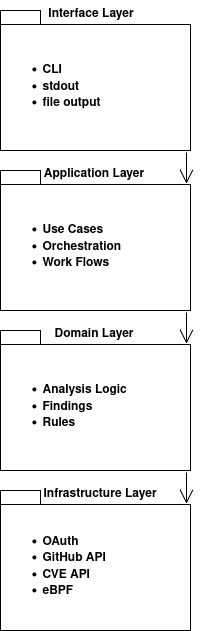
\includegraphics[scale=0.5, keepaspectratio]{images/high-level-layers}
\caption{High Level Layers}
\end{figure}

The Hexagonal Architecture is used to bring the layers to life and substantiate the aspects of each layer.

\subsubsection{Hexagonal Architecture}

The Hexagonal Architecture adheres to the Separation of Concern principle. It is also referred to as the Ports and Adapters architecture. The main goal is to create abstraction layers resulting in isolation of the core business logic and any outside concerns and components(database, external APIs, frameworks etc.).\newline The architecture has an elegant solution for the flow of data. The input of data which can originate from a user or other external service passes into the application at a port using an adapter. The output reverses the flow of data and goes from the application to an apdapter through the port \footnote{Pablo Martinez. Hexagonal Architecture, there are always two sides to every story. [online] homepage: medium.com URL: https://medium.com/ssense-tech/hexagonal-architecture-there-are-always-two-sides-to-every-story-bc0780ed7d9c [Accessed 08.01.2026]}.

\subsection{Component Design}

!

\subsection{UML Diagram}

Maybe Use Case Diagram, Activity Diagram

\subsection{Data Flow}

\subsubsection{Description}

\subsubsection{Flowchart}

\subsection{User Interface Design}

The tool has a command line interface (CLI). The Typer library will be used to build the CLI. The following code shows an outline of the structure:

\subsubsection{CLI Menu}

The CLI has various flags for options to choose from:

\begin{itemize}
	\item -s flag: statical mode for statical analysis
	\item -b flag: behavioral mode for behavioral analysis
	\item -u flag: ultimate mode, for both statical and behavioral analysis
	\item -r flag: generates a report text file of the findings (default output is stdout)
\end{itemize}

\subsection{Security Considerations}

\subsection{Design Decisions and Rationale}

\subsubsection{Hexagonal Architecture}

\footnote{URL: https://dev.to/dyarleniber/hexagonal-architecture-and-clean-architecture-with-examples-48oi}
\footnote{URL: https://senseisrl.it/en/tech-tales/hexagonal-architecture-principles-and-benefits}

\subsection{Limitations}

\subsubsection{Edge Cases}

\subsubsection{Future Improvements}

\section{Implementation}

\subsection{Introduction}

!

\subsection{Development Environment}

!

\subsection{System Setup / Dependencies}

!

\subsection{Implementation Overview}

!

\subsection{Key Components}

!

\subsection{Error Handling \& Logging}

!

\subsection{Security Aspects in Implementation}

!

\subsection{Challenges during Implementation}

!

\section{Utilization}

The utilization chapter goes through a specific use case, explains in detail how to use the tool and the output it produces. It furthers talks about limitations and aspects in regards to perfomance. 

\subsection{Use Cases}

\textbf{Scenario}: The user wants to run the static analysis on a Linux machine and have the results displayed on the console.

\subsection{Execution: Step-by-step Guide}

Here is a step by step discription how the use case is played out.

\subsubsection{Open terminal and execute Python package}

It is a CLI tool and therefore it is mandatory to use the terminal for the tool to work. Once everything is set up properly the tool is run by writing "linux-analyzer" on the command line and pressing enter.

\smallskip
\begin{figure}[h]
\centering
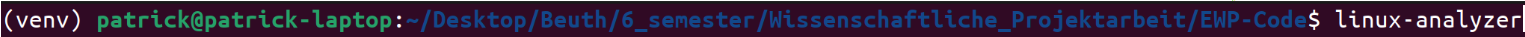
\includegraphics[scale=0.3, keepaspectratio]{images/linux-analyzer-cmd-line-exec}
\caption{Tool Execution - Command Line}
\end{figure}

If everything works and the tool starts up properly a prompt will be visible next. It asks the user to choose a mode for the analysis and if applicable the report or/and cve option.

\smallskip
\begin{figure}[h]
\centering
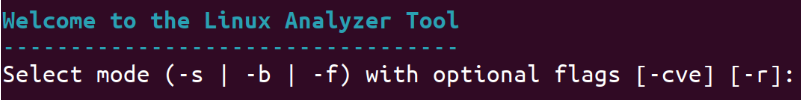
\includegraphics[scale=0.3, keepaspectratio]{images/user-input-prompt}
\caption{Prompt for user input}
\end{figure}

After picking the flags the program runs with the chosen settings.\newline Insert pick during runtime!


\subsection{Output Interpretation}

The output of the analysis is displayed on the console as the default configuration. The user can use the optional -r flag when executing the tool to generate a report in text file format. \newline The content and meaning of the ouput is dependent on the mode and optional flags chosen by the user. 

\subsubsection{Example Outputs}

\subsection{Limitations in Usage}

There are certain limitations in place. It is a CLI tool, therefore it has to be started from the command line. This is non-negotiable and the only way to use the tool. \newline The tool solely runs on machines which have a Linux distribution as there operating system.

\subsubsection{Permissions and Rights}

The tool handles highly sensitive data. This is why getting the permissions and rights exactly right is of paramount importance. Consequently running the entire tool with root privileges is out of question. The goal is to have a nuanced approach and identify the exact areas and which need elevated privileges. This scenario calls for the security design principle referred to as privilege separation. Each component of the application has tailored and distinct privileges according to its needs and tasks. No component has more privileges than it needs to do its designated jobs.\newline 

The static analysis does not need root privileges. It needs read access to files and certain folders including \textit{/user/bin}, \textit{/etc} among others. It may need elevated read access on hardened systems but is can be solved through group membership, read-only ACLs and capabilities.\newline 

The behavioral part of the analysis is a different story though. Runtime analysis requires root or near-root privileges in regards to syscall tracing, eBPF, network inspection and kernel/process introspection. It is important to note that some will run as actual root while others will use a dedicated system user with specific capabilities whenever possible.

\subsection{Performance}

\subsubsection{Execution Time}

\subsubsection{Statisitcs and Benchmarking}

\section{Evaluation}

\subsection{Introduction}

!

\subsection{Metric for Evaluation}

!

\subsection{Overview of Tests and Setup}

!

\subsection{Tests and and Analysis}

!

\subsection{Quantitative Results}

!

\subsection{User Feedback}

!


\section{Appendix}


%\smallskip
%\begin{figure}[h]
%\centering
%\includegraphics[scale=0.3, keepaspectratio]{gantt}
%\caption{Timetable: Gantt-Diagram}
%\end{figure}

\newpage

\bibliographystyle{is-plain}
\nocite{*}
\bibliography{bib/project-refs}


\end{document}





